\documentclass[11pt]{article}
\usepackage[a4paper,margin=2.2cm]{geometry}
\usepackage[T1]{fontenc}
\usepackage{lmodern}
\usepackage{amsmath,amssymb}
\usepackage{xcolor}
\usepackage{graphicx}
\usepackage{titlesec}
\usepackage{enumitem}
\usepackage[most]{tcolorbox}

\definecolor{hd}{RGB}{20,60,130}
\definecolor{kw}{RGB}{120,60,0}
\titleformat{\section}{\color{hd}\Large\bfseries}{}{0pt}{}
\titleformat{\subsection}{\color{hd}\bfseries}{}{0pt}{}
\titlespacing*{\subsection}{0pt}{10pt}{4pt}
\setlength{\parindent}{0pt}
\setlength{\parskip}{5pt}
\setlist{nosep,itemsep=2pt}

\newcommand{\pd}{\partial}
\newcommand{\bu}{\mathbf u}
\newcommand{\bo}{\boldsymbol\omega}
\newcommand{\kw}[1]{{\color{kw}\itshape ``#1''}}
\newtcolorbox{strategy}{colback=hd!5,colframe=hd!60,boxrule=0.5pt,arc=2pt,left=5pt,right=5pt,top=3pt,bottom=3pt,fonttitle=\bfseries\small,title=Strategy}
\newcommand{\why}[1]{{\color{gray}\small[#1]}}

\begin{document}
\begin{center}
{\color{hd}\Large\bfseries Physics of Fluids (PHYSFLU) --- Midterm Exam 2020--2021}\\[3pt]
Detailed resolution
\end{center}

%==================================================================
\section*{Problem 1 \normalsize(2 p.)}

\begin{strategy}
We are given a stream function $\psi$. Velocities follow from $u=\pd_y\psi$, $v=-\pd_x\psi$.
\kw{incompressible} $\to$ check $\nabla\!\cdot\bu=0$. \kw{irrotational?} $\to$ compute $\omega_z=-\nabla^2\psi$.
For the pressure: if the flow is irrotational, Bernoulli holds between \emph{any} two points, so we can link any point on the wall with the reference point $(0,0)$.
\end{strategy}

Write $\psi=A\left(e^{-ky}-e^{ky}\right)\sin kx=-2A\sinh(ky)\sin(kx)$, using $e^{ky}-e^{-ky}=2\sinh ky$. The velocity components are
\[
u=\frac{\pd\psi}{\pd y}=-2Ak\cosh(ky)\sin(kx),\qquad
v=-\frac{\pd\psi}{\pd x}=2Ak\sinh(ky)\cos(kx).
\]
Note that $\psi(x,0)=0$ for all $x$: the plane $y=0$ is a streamline, so the flow does not cross the wall, as it must ($v(x,0)=0$). The wavy wall near $y=H$ is another streamline, $\psi=$ const.

\subsection*{(a) Continuity}
For an incompressible flow, mass conservation reduces to $\nabla\!\cdot\bu=0$:
\[
\frac{\pd u}{\pd x}+\frac{\pd v}{\pd y}
=-2Ak^2\cosh(ky)\cos(kx)+2Ak^2\cosh(ky)\cos(kx)=0 .
\]
Yes, the continuity equation is satisfied. This is no accident: for \emph{any} $\psi$, $\pd_xu+\pd_yv=\pd_x\pd_y\psi-\pd_y\pd_x\psi=0$, because mixed partial derivatives commute. A 2D velocity field built from a stream function is always divergence-free.

\subsection*{(b) Irrotationality}
The only non-zero vorticity component in a 2D flow is
\[
\omega_z=\frac{\pd v}{\pd x}-\frac{\pd u}{\pd y}=-\left(\frac{\pd^2\psi}{\pd x^2}+\frac{\pd^2\psi}{\pd y^2}\right)=-\nabla^2\psi .
\]
Since $\pd_x^2\psi=-k^2\psi$ (from $\sin kx$) and $\pd_y^2\psi=+k^2\psi$ (from $\sinh ky$),
\[
\nabla^2\psi=-k^2\psi+k^2\psi=0\quad\Longrightarrow\quad\omega_z=0 .
\]
The flow is irrotational. Equivalently, $\psi$ is harmonic, so a velocity potential $\phi$ exists with $\bu=\nabla\phi$ (here $\phi=2A\cosh(ky)\cos(kx)$, which satisfies $\pd_x\phi=u$, $\pd_y\phi=v$).

\subsection*{(c) Pressure on the plane wall $y=0$}
\textbf{Which equation?} $\psi$ does not depend on $t$, so the flow is steady; it is incompressible and irrotational, and gravity is neglected. Under these conditions
\[
\frac{p}{\rho}+\frac12|\bu|^2=\text{const}\quad\text{in the whole domain}
\]
(Bernoulli from Euler: $\bo\times\bu=-\nabla H$ with $\bo=0$ gives $\nabla H=0$.)
\why{Even if the fluid were viscous, the viscous term $\nu\nabla^2\bu=-\nu\nabla\times\bo$ vanishes for an irrotational incompressible flow, so the result does not change.}

\textbf{Velocity on the wall.} At $y=0$: $\cosh 0=1$, $\sinh 0=0$, so
\[
u(x,0)=-2Ak\sin(kx),\qquad v(x,0)=0,\qquad |\bu|^2=4A^2k^2\sin^2(kx).
\]

\textbf{Fix the constant with the reference point.} At $(0,0)$: $u=0$ (since $\sin 0=0$), $v=0$, and $p=0$. Hence the Bernoulli constant is $0$:
\[
p(x,0)+\frac{\rho}{2}\,4A^2k^2\sin^2(kx)=0
\quad\Longrightarrow\quad
\boxed{\,p(x,0)=-2\rho A^2k^2\sin^2(kx)\,}
\]
\textbf{Interpretation.} The origin is a stagnation point, where the pressure is maximum. Along the wall the fluid accelerates and the pressure drops, reaching its minimum $-2\rho A^2k^2$ where $|u|$ is largest, at $kx=\pm\pi/2$. The pattern repeats every $\pi/k$, half a wavelength of the wavy wall.

%==================================================================
\section*{Problem 2 \normalsize(2 p.)}

\begin{strategy}
\kw{incompressible} in this course means that the density of each fluid particle does not change: $\dfrac{D\rho}{Dt}=0$. We are given $\rho(x,y,z,t)$, so we compute its material derivative and force it to vanish: this gives $f(t)$.
Pathlines: integrate $\dot{\mathbf x}=\bu(\mathbf x,t)$ with the initial position.
Circulation: either the line integral of $\bu$ around the circle, or the flux of vorticity (Stokes).
\end{strategy}

\subsection*{(a) Determining $f(t)$}
The material derivative is $\dfrac{D\rho}{Dt}=\pd_t\rho+u\,\pd_x\rho+v\,\pd_y\rho+w\,\pd_z\rho$. Term by term, with $\rho=e^{-2t}(x^2+y^2)+z^2e^{-t^2}+C$:
\begin{align*}
\pd_t\rho&=-2e^{-2t}(x^2+y^2)-2t\,z^2e^{-t^2},\\
u\,\pd_x\rho+v\,\pd_y\rho&=x\cdot2xe^{-2t}+y\cdot2ye^{-2t}=2e^{-2t}(x^2+y^2),\\
w\,\pd_z\rho&=z f(t)\cdot2ze^{-t^2}=2f(t)\,z^2e^{-t^2}.
\end{align*}
Adding, the $(x^2+y^2)$ terms cancel and
\[
\frac{D\rho}{Dt}=2z^2e^{-t^2}\big(f(t)-t\big)=0\ \ \forall z
\quad\Longrightarrow\quad \boxed{f(t)=t}
\]
\why{Remark: with $f=t$ one finds $\nabla\!\cdot\bu=2+t\neq0$, so the full continuity equation $D\rho/Dt+\rho\nabla\!\cdot\bu=0$ is not strictly satisfied. The statement is not fully consistent; the intended route is $D\rho/Dt=0$, as above.}

\subsection*{(b) Pathlines}
A pathline is the trajectory $\mathbf x(t)$ of one particle: $\dot x=u$, $\dot y=v$, $\dot z=w$, starting from $(x_0,y_0,z_0)$ at $t=0$. Each equation is separable:
\begin{align*}
\frac{dx}{dt}=x &\ \Rightarrow\ \int_{x_0}^{x}\frac{dx}{x}=\int_0^tdt\ \Rightarrow\ x=x_0e^{t},\\
\frac{dy}{dt}=y &\ \Rightarrow\ y=y_0e^{t},\\
\frac{dz}{dt}=t\,z &\ \Rightarrow\ \ln\frac{z}{z_0}=\frac{t^2}{2}\ \Rightarrow\ z=z_0e^{t^2/2}.
\end{align*}
To get the \emph{curve}, eliminate $t$ using $t=\ln(x/x_0)$:
\[
\boxed{\ \frac{y}{y_0}=\frac{x}{x_0},\qquad z=z_0\exp\!\left[\tfrac12\ln^2\!\left(\frac{x}{x_0}\right)\right]\ }
\]
The particle moves radially outward in the $x$--$y$ plane (straight line through the origin), while its height grows faster and faster. Since the flow is unsteady ($w$ depends on $t$), these pathlines do \emph{not} coincide with the streamlines.

\subsection*{(c) Circulation around the circle $x^2+y^2=a^2$ in the $x$--$y$ plane}
\textbf{Route 1 (line integral).} On the circle $\bu=(x,y,\cdot)$ is purely radial in the plane, $\bu_\parallel=r\,\hat r$, while $d\mathbf l=a\,d\theta\,\hat\theta$. Thus $\bu\cdot d\mathbf l=0$ at every point and
\[
\Gamma=\oint\bu\cdot d\mathbf l=0 .
\]
\textbf{Route 2 (Stokes).} $\omega_z=\pd_xv-\pd_yu=\pd_x(y)-\pd_y(x)=0$, so $\Gamma=\int_S\omega_z\,dS=0$. In fact all components of $\bo$ vanish ($w$ depends only on $z$, $t$), so the flow is irrotational. \quad $\boxed{\Gamma=0}$

%==================================================================
\section*{Problem 3 \normalsize(3 p.)}

\begin{strategy}
Keywords: \kw{steadily}, \kw{fully developed}, \kw{constant width}, \kw{axisymmetry}, \kw{no pressure gradient in $z$} $\Rightarrow$ $\pd_t=0$, $\pd_z\bu=0$, $\pd_\theta=0$, $\pd_zp=0$, $\bu=u_z(r)\hat z$.
Only the $z$-momentum equation is non-trivial; it is driven by gravity. Boundary conditions: \kw{solid cylinder at rest} $\to$ no slip at $r=a$; \kw{film} in contact with air $\to$ free surface, zero shear stress at $r=b$.
Temperature: the energy equation reduces to conduction balancing viscous dissipation. BCs: $T=T_w$ at the cylinder, no heat flux through the free surface.
\end{strategy}

\textbf{Axes.} $z$ points downwards (as in the figure), so gravity is $\mathbf g=+g\hat z$ and the film flows in $+z$.

\subsection*{(a) Velocity profile}
\textbf{Step 1: simplify.} With $\bu=u_z(r)\hat z$: continuity, $\pd_zu_z=0$, is satisfied identically. The $r$- and $\theta$-components of NS give $\pd_rp=0$ and $\pd_\theta p=0$ (no $u_r$, $u_\theta$), consistent with $p=p_a$. In the $z$-component, the convective term $(\bu\cdot\nabla)u_z=u_z\pd_zu_z=0$, $\pd_tu_z=0$ and $\pd_zp=0$, leaving
\[
0=\rho g+\mu\,\frac1r\frac{d}{dr}\!\left(r\frac{du_z}{dr}\right).
\]
\why{Gravity (the driving force) is balanced by viscous friction transmitted across cylindrical layers.}

\textbf{Step 2: integrate twice.}
\[
\frac{d}{dr}\!\left(r\,u_z'\right)=-\frac{\rho g}{\mu}r
\ \Rightarrow\
r\,u_z'=-\frac{\rho g}{2\mu}r^2+C_1
\ \Rightarrow\
u_z=-\frac{\rho g}{4\mu}r^2+C_1\ln r+C_2 .
\]
The point $r=0$ is \emph{not} in the fluid domain ($a\le r\le b$), so the $\ln r$ solution must be kept.

\textbf{Step 3: boundary conditions.}
\begin{itemize}
\item Free surface, $r=b$: the air exerts negligible shear, $\tau_{rz}=\mu\,u_z'(b)=0$:
\[
-\frac{\rho g}{2\mu}b+\frac{C_1}{b}=0\ \Rightarrow\ C_1=\frac{\rho g b^2}{2\mu}.
\]
\item No slip on the cylinder at rest, $u_z(a)=0$: $C_2=\frac{\rho g}{4\mu}a^2-C_1\ln a$.
\end{itemize}
Substituting,
\[
\boxed{\,u_z(r)=\frac{\rho g}{4\mu}\left(a^2-r^2\right)+\frac{\rho g b^2}{2\mu}\ln\frac{r}{a}\,}
\qquad\Longrightarrow\qquad
\alpha=\frac{\rho g}{4\mu},\quad \beta=\frac{\rho g b^2}{2\mu}.
\]
\textbf{Check.} $u_z'=\frac{\rho g}{2\mu}\frac{b^2-r^2}{r}>0$ for $r<b$: the velocity grows from 0 at the wall to its maximum at the free surface, and it is positive (downwards), as expected. For a thin film ($b-a\ll a$) it reduces to the half-parabola of a film on a vertical plate.

\subsection*{(b) Temperature profile}
\textbf{Step 1: simplify the energy equation.} Steady and fully developed means $T=T(r)$, so the convective term $\bu\cdot\nabla T=u_z\pd_zT=0$. What remains is a balance between heat conduction and viscous dissipation $\Phi$:
\[
0=\lambda\frac1r\frac{d}{dr}\!\left(r\frac{dT}{dr}\right)+\Phi,\qquad
\Phi=\mu\left(\frac{du_z}{dr}\right)^2=\frac{\rho^2g^2}{4\mu}\,\frac{\left(b^2-r^2\right)^2}{r^2}.
\]

\textbf{Step 2: first integration.} Multiply by $r/\lambda$ and expand $\frac{(b^2-r^2)^2}{r}=\frac{b^4}{r}-2b^2r+r^3$:
\[
\frac{d}{dr}\!\left(rT'\right)=-\frac{\rho^2g^2}{4\mu\lambda}\left(\frac{b^4}{r}-2b^2r+r^3\right)
\ \Rightarrow\
rT'=-\frac{\rho^2g^2}{4\mu\lambda}\left(b^4\ln r-b^2r^2+\frac{r^4}{4}\right)+C_3 .
\]

\textbf{Step 3: BC at the free surface.} The air is a poor conductor, so no heat crosses the surface: $T'(b)=0$. This gives $C_3=\frac{\rho^2g^2}{4\mu\lambda}\left(b^4\ln b-\frac34b^4\right)$, so
\[
rT'=-\frac{\rho^2g^2}{4\mu\lambda}\left[b^4\ln\frac rb-b^2r^2+\frac{r^4}{4}+\frac34b^4\right].
\]

\textbf{Step 4: second integration and BC $T(a)=T_w$.} Divide by $r$ and integrate from $a$ to $r$, using $\int\frac{\ln(r/b)}{r}dr=\frac12\ln^2\frac rb$:
\[
\boxed{\,T(r)=T_w+\frac{\rho^2g^2}{4\mu\lambda}\left[\frac{b^2}{2}\left(r^2-a^2\right)-\frac{r^4-a^4}{16}-\frac{b^4}{2}\ln\frac ra\,\ln\frac{ra}{b^2}-\frac34b^4\ln\frac ra\right]}
\]
(using $\ln^2\frac rb-\ln^2\frac ab=\ln\frac ra\ln\frac{ra}{b^2}$).

\textbf{Interpretation.} Friction heats the film. The heat cannot escape through the free surface, so it all flows into the cylinder. Therefore $T$ increases from $T_w$ at the wall to its maximum at the free surface (where $T'=0$), see the figure. Energy check: the heat flux into the wall per unit length, $2\pi a\lambda T'(a)$, equals the total dissipation $\int_a^b2\pi r\Phi\,dr$, which is in turn the work done by gravity on the falling film.

\begin{center}
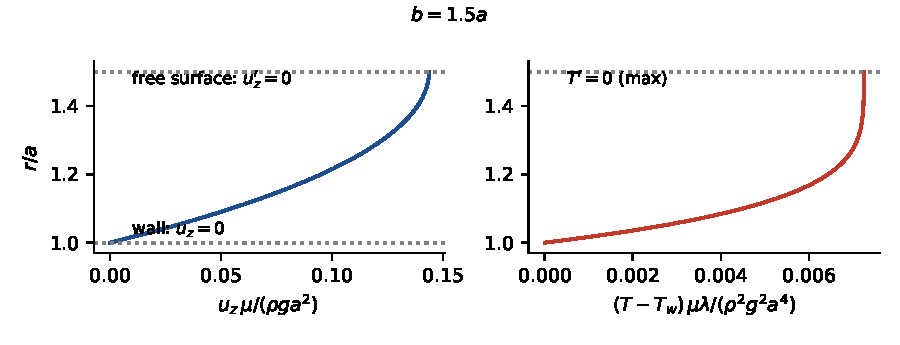
\includegraphics[width=0.85\textwidth]{qt20_p3.pdf}
\end{center}

%==================================================================
\section*{Problem 4 \normalsize(3 p.)}

\begin{strategy}
Keywords: \kw{steadily}, \kw{infinite plates}, \kw{two-dimensional}, $w=0$ $\Rightarrow$ $\pd_t=0$, $\pd_x\bu=0$ (but $\pd_xp=-K\ne0$).
\kw{porous}, \kw{$v=-v_0$ at each plate} $\Rightarrow$ continuity forces $v=-v_0$ everywhere. Unlike the classic Poiseuille flow, the convective term $v\,\pd_yu$ does \emph{not} vanish, which gives a 2nd-order ODE with constant coefficients.
BCs: plates at rest $\to$ $u(0)=u(h)=0$ (no slip for the tangential component).
\end{strategy}

\textbf{Step 1: continuity.} $\pd_xu+\pd_yv=0$ with $\pd_xu=0$ (fully developed) gives $\frac{dv}{dy}=0$. So $v$ is constant and equal to its wall value:
\[
v(y)=-v_0\quad\text{for all }0\le y\le h .
\]
The fluid enters through the upper plate and leaves through the lower one.

\textbf{Step 2: $y$-momentum.} $\rho\left(u\pd_xv+v\pd_yv\right)=-\pd_yp+\mu\nabla^2v$. Every velocity term vanishes ($v$ is constant), so $\pd_yp=0$. Together with $\pd_xp=-K$:
\[
p=p_0-Kx .
\]

\textbf{Step 3: $x$-momentum.}
\[
\rho\Big(\underbrace{u\pd_xu}_{0}+v\,\pd_yu\Big)=-\pd_xp+\mu\pd_y^2u
\ \Rightarrow\
-\rho v_0u'=K+\mu u''
\ \Rightarrow\
u''+\frac{v_0}{\nu}u'=-\frac{K}{\mu}.
\]

\textbf{Step 4: solve the ODE.} It is linear with constant coefficients, so $u=u_h+u_p$.
\begin{itemize}
\item Homogeneous: try $e^{\lambda y}$, $\lambda^2+\frac{v_0}{\nu}\lambda=0\Rightarrow\lambda=0,\ -\frac{v_0}{\nu}$. So $u_h=C_1+C_2e^{-v_0y/\nu}$.
\item Particular: the right-hand side is a constant, but $\lambda=0$ is already a root, so try $u_p=cy$: $\frac{v_0}{\nu}c=-\frac K\mu\Rightarrow c=-\frac{K}{\rho v_0}$.
\end{itemize}
\[
u=C_1+C_2e^{-v_0y/\nu}-\frac{K}{\rho v_0}y .
\]

\textbf{Step 5: BCs.} From $u(0)=0$: $C_2=-C_1$. From $u(h)=0$: $C_1\left(1-e^{-v_0h/\nu}\right)=\frac{Kh}{\rho v_0}$. Hence
\[
\boxed{\ u(y)=\frac{K}{\rho v_0}\left[h\,\frac{1-e^{-v_0y/\nu}}{1-e^{-v_0h/\nu}}-y\right],\qquad v=-v_0,\qquad w=0\ }
\]

\textbf{Checks and interpretation.}
\begin{itemize}
\item \emph{Limit $v_0\to0$.} Expanding $e^{-s}\simeq1-s+s^2/2$ gives $u\to\frac{K}{2\mu}y(h-y)$, the plane Poiseuille flow. \checkmark
\item \emph{Strong suction, $R=v_0h/\nu\gg1$.} The suction pushes momentum towards the lower plate. The profile becomes almost linear, $u\simeq\frac{K}{\rho v_0}(h-y)$, except in a thin layer of thickness $\nu/v_0$ near $y=0$ where it drops to zero (see the figure). The maximum moves towards the lower plate.
\end{itemize}
\begin{center}
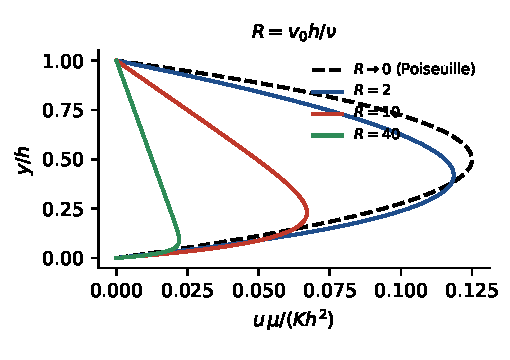
\includegraphics[width=0.5\textwidth]{qt20_p4.pdf}
\end{center}

\end{document}
